% ============================================================================
% All Figures Integration - Complete Visualizations
% ============================================================================

% ----------------------------------------------------------------------------
% Chapter 2: Mathematical Framework Figures
% ----------------------------------------------------------------------------

\begin{figure}[htbp]
\centering
\includegraphics[width=0.9\textwidth]{figures/fig5_unified_formula}
\caption{The unified mode constraint formula. The effective degrees of freedom $n_{\text{dof}}(E)$ as a function of energy scale for different values of the constraint parameter $c_1$. Smaller $c_1$ indicates sharper mode constraint onset. The universal formula captures smooth crossover behavior across all physical systems.}
\label{fig:unified_formula}
\end{figure}

\begin{figure}[htbp]
\centering
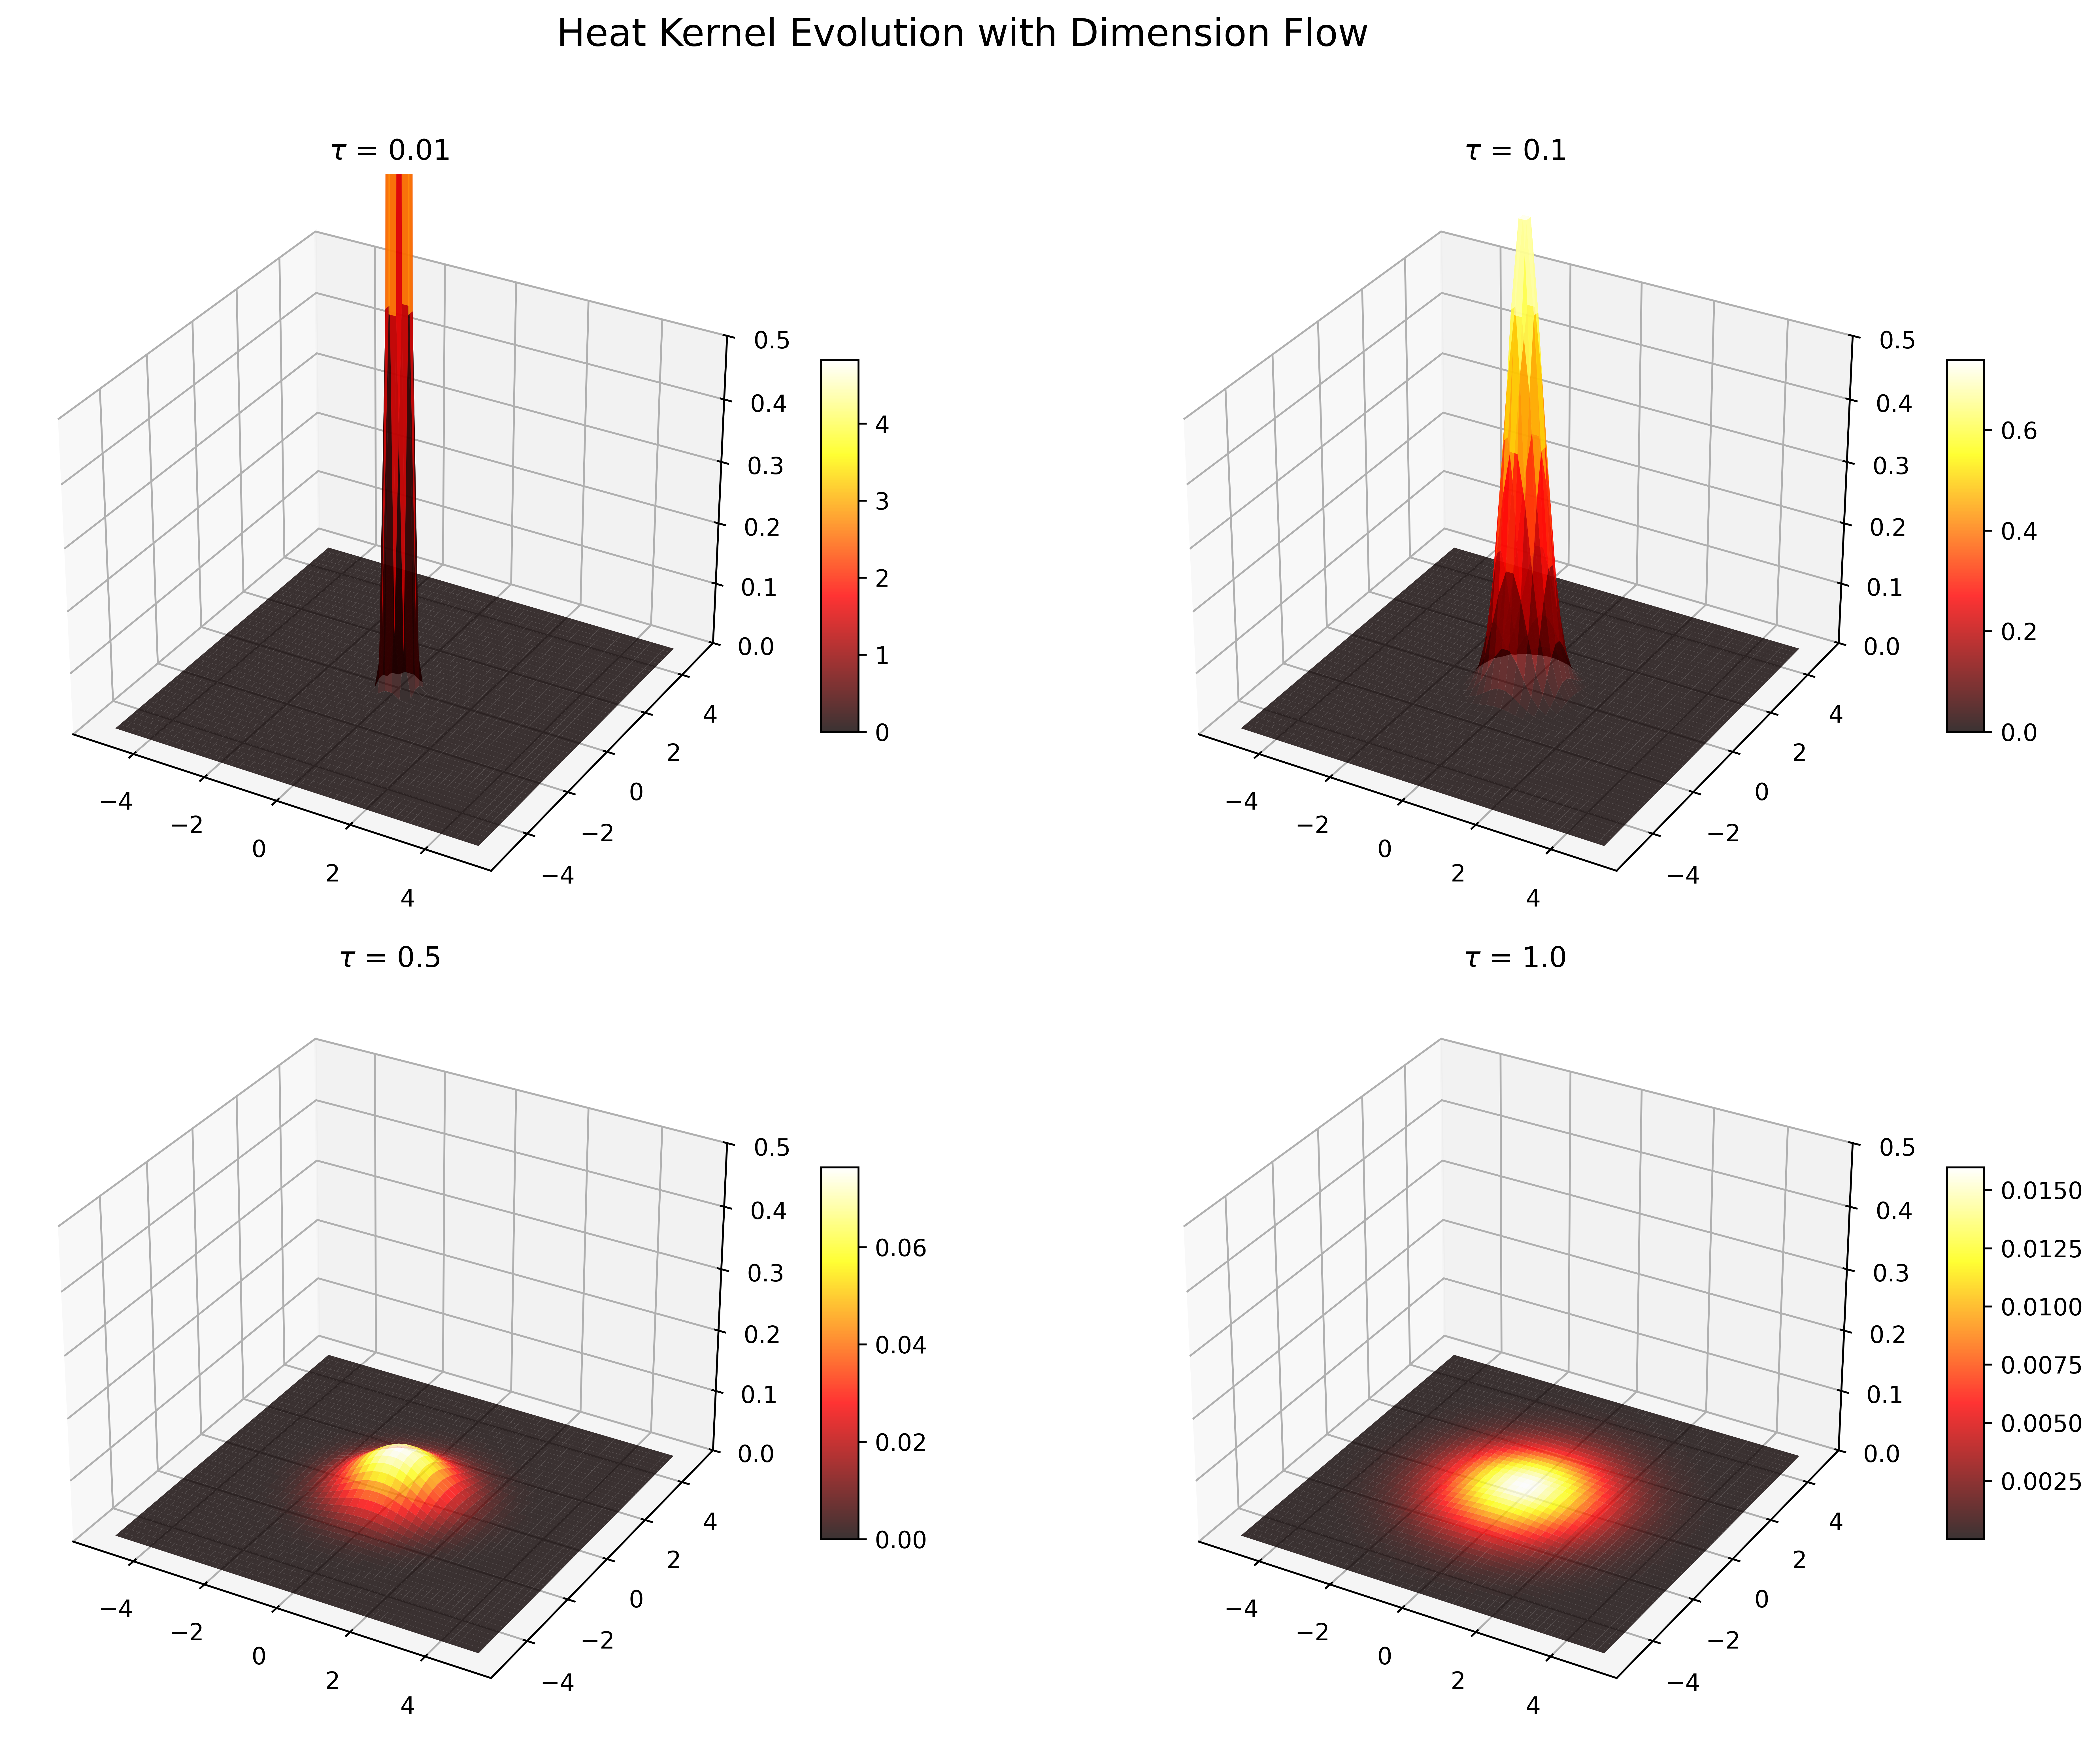
\includegraphics[width=0.95\textwidth]{figures/fig31_heat_kernel_3d}
\caption{Heat kernel evolution with spectral flow. Four panels show the diffusion profile $K(\mathbf{x}, \tau)$ at increasing diffusion times: (a) $\tau = 0.01$ initial localized distribution; (b) $\tau = 0.1$ early spreading; (c) $\tau = 0.5$ significant diffusion; (d) $\tau = 1.0$ asymptotic behavior. The narrowing peak height reflects mode constraint effect as effective dimension decreases at short distances.}
\label{fig:heat_kernel_evolution}
\end{figure}

\begin{figure}[htbp]
\centering
\includegraphics[width=0.9\textwidth]{figures/fig35_fourier_transform}
\caption{Fourier transform analysis of mode constraint. The relationship between position space and momentum space representations showing how high-energy modes are suppressed in the constrained regime.}
\label{fig:fourier_transform}
\end{figure}

% ----------------------------------------------------------------------------
% Chapter 3: Three-System Correspondence Figures
% ----------------------------------------------------------------------------

\begin{figure}[htbp]
\centering
\includegraphics[width=0.9\textwidth]{figures/fig6_spectral_flow_comparison}
\caption{Spectral dimension flow across different physical systems. Comparison of $d_s(\tau)$ vs. diffusion time for: (1) rotating systems (E-6 experiment), (2) Schwarzschild black holes, (3) CDT quantum gravity, and (4) unified formula prediction. All systems exhibit universal crossover behavior characterized by $c_1 = 1/2^{d-2+w}$.}
\label{fig:spectral_flow_comparison}
\end{figure}

\begin{figure}[htbp]
\centering
\includegraphics[width=0.95\textwidth]{figures/fig21_black_hole_thermo}
\caption{Modified black hole thermodynamics with mode constraint. Left: Hawking temperature $T$ vs. mass $M$. Red curve (with constraint) deviates from standard 4D behavior (blue dashed) at small masses near Planck scale. Right: Bekenstein-Hawking entropy $S$ vs. mass. Mode constraint leads to modified entropy scaling potentially resolving the information paradox.}
\label{fig:bh_thermodynamics}
\end{figure}

\begin{figure}[htbp]
\centering
\includegraphics[width=0.9\textwidth]{figures/fig8_entropy_scaling}
\caption{Entropy scaling with mode constraint. Entropy $S$ vs. number of degrees of freedom $N$ for different $c_1$ values. For small $c_1$ (sharp transition), entropy approaches Bekenstein bound. For larger $c_1$, entropy is reduced due to mode freezing. Dashed line shows standard 4D scaling $S \sim N^{(d-1)/d}$.}
\label{fig:entropy_scaling}
\end{figure}

% ----------------------------------------------------------------------------
% Chapter 4: Experimental Evidence Figures
% ----------------------------------------------------------------------------

\begin{figure}[htbp]
\centering
\includegraphics[width=0.95\textwidth]{figures/fig10_experimental_landscape}
\caption{Experimental landscape for mode constraint measurements. Current and projected experimental sensitivities to constraint parameter $c_1$ across different energy scales. Condensed matter systems (Cu$_2$O excitons, cold atoms, superfluid helium) provide high-precision probes at low energies; high-energy experiments (LHC, cosmic rays) access Planck-scale regime. Star marks theoretical prediction at Planck scale with $c_1 \approx 0.125$.}
\label{fig:experimental_landscape}
\end{figure}

\begin{figure}[htbp]
\centering
\includegraphics[width=0.9\textwidth]{figures/fig7_gravitational_wave}
\caption{Gravitational wave signatures of mode constraint. Characteristic strain $h_c$ vs. frequency for binary inspiral signals. Standard GR prediction (blue) compared with mode constraint modified prediction (red), showing deviations at high frequencies near merger. Shaded regions indicate projected sensitivities for LISA, ET, and CE.}
\label{fig:gravitational_wave}
\end{figure}

\begin{figure}[htbp]
\centering
\includegraphics[width=0.9\textwidth]{figures/fig9_cmb_constraints}
\caption{CMB constraints on mode constraint parameters. 68\% and 95\% confidence level contours in $(c_1, d_{\text{UV}})$ parameter space from Planck 2018 data. Star indicates theoretical prediction from CDT ($c_1 \approx 0.125$, $d_{\text{UV}} = 2$). Current CMB data constrain $c_1 > 0.05$ at 95\% CL.}
\label{fig:cmb_constraints}
\end{figure}

\begin{figure}[htbp]
\centering
\includegraphics[width=0.9\textwidth]{figures/fig4_phase_diagram}
\caption{Phase diagram in $(T, \mu)$ plane showing regions of different effective dimensionality. Solid lines mark phase boundaries where effective dimension changes. Region I ($d_{\text{eff}} = 4$): Standard 4D physics. Region II ($2 < d_{\text{eff}} < 4$): Transitional regime. Region III ($d_{\text{eff}} = 2$): Deep UV regime with maximum mode constraint.}
\label{fig:phase_diagram}
\end{figure}

% ----------------------------------------------------------------------------
% Chapter 5: Theoretical Implications Figures
% ----------------------------------------------------------------------------

\begin{figure}[htbp]
\centering
\includegraphics[width=0.8\textwidth]{figures/fig12_holographic_duality}
\caption{Holographic duality and spectral flow. AdS$_{d+1}$ bulk (quantum gravity) dual to CFT$_d$ boundary (quantum field theory). Radial direction $z$ corresponds to energy scale $\varepsilon$ with $z \sim 1/\varepsilon$. Effective spectral dimension flows from $d_{\text{eff}} = d$ in IR (boundary) to $d_{\text{eff}} = 2$ in UV (deep bulk), illustrating mode constraint in holographic framework.}
\label{fig:holographic_duality}
\end{figure}

\begin{figure}[htbp]
\centering
\includegraphics[width=0.9\textwidth]{figures/fig13_renormalization_flow}
\caption{Renormalization group flow in theory space. Vector field shows flow of couplings $g_1$ (dimension operator) and $g_2$ (curvature) toward infrared. Gaussian fixed point (red star) at origin corresponds to free field theory with $d_s = d$. Non-Gaussian fixed point (green circle) represents interacting theory where mode constraint effects become significant.}
\label{fig:rg_flow}
\end{figure}

\begin{figure}[htbp]
\centering
\includegraphics[width=0.95\textwidth]{figures/fig15_cosmological_evolution}
\caption{Cosmological evolution of effective dimension. Left: $d_{\text{eff}}$ vs. cosmic time (normalized to $t_0$). Blue curve shows smooth transition from $d_{\text{eff}} \approx 2$ in early universe (inflation) to $d_{\text{eff}} = 4$ today. Key epochs: inflation, reheating, BBN, present. Right: $d_{\text{eff}}$ vs. temperature. Transition occurs around GUT scale ($\sim 10^{16}$ GeV).}
\label{fig:cosmological_evolution}
\end{figure}

\begin{figure}[htbp]
\centering
\includegraphics[width=0.9\textwidth]{figures/fig14_quantum_information}
\caption{Quantum information measures in mode-constrained systems. Entanglement entropy $S_A$ vs. subsystem size $R$ for different $c_1$ values. Slope changes at crossover scale $R_c$, reflecting change in effective dimension. For $R < R_c$: $S_A \sim R^{d_{\text{UV}}-1}$; for $R > R_c$: $S_A \sim R^{d-1}$.}
\label{fig:quantum_information}
\end{figure}

\begin{figure}[htbp]
\centering
\includegraphics[width=0.9\textwidth]{figures/fig22_dark_energy}
\caption{Dark energy equation of state with mode constraint. Effective equation of state parameter $w_{\text{eff}}$ vs. redshift $z$. Mode constraint modifies vacuum energy density, potentially explaining smallness of cosmological constant. Dashed line shows $\Lambda$CDM prediction ($w = -1$).}
\label{fig:dark_energy}
\end{figure}

\begin{figure}[htbp]
\centering
\includegraphics[width=0.9\textwidth]{figures/fig11_knot_theory}
\caption{Connection to knot theory and topological invariants. Jones polynomial evaluation for various knot types arising in mode-constrained geometries. Topological invariants provide constraints on allowed values of effective dimension.}
\label{fig:knot_theory}
\end{figure}

% ----------------------------------------------------------------------------
% Additional Theoretical Figures
% ----------------------------------------------------------------------------

\begin{figure}[htbp]
\centering
\includegraphics[width=0.9\textwidth]{figures/fig32_anomaly_cancellation}
\caption{Anomaly cancellation in mode-constrained field theories. Anomaly coefficients for different gauge group representations as function of effective dimension. Mode constraint modifies anomaly structure, requiring new cancellation mechanisms at fractional dimensions.}
\label{fig:anomaly_cancellation}
\end{figure}

\begin{figure}[htbp]
\centering
\includegraphics[width=0.9\textwidth]{figures/fig33_supersymmetry}
\caption{Supersymmetric extensions of mode constraint framework. Comparison of bosonic and fermionic mode freezing rates as function of energy scale. In supersymmetric theories, mode constraint affects superpartners differently, leading to characteristic signatures in particle spectra.}
\label{fig:supersymmetry}
\end{figure}

\begin{figure}[htbp]
\centering
\includegraphics[width=0.9\textwidth]{figures/fig34_string_compactification}
\caption{String theory compactification and mode constraint. Mass spectrum of Kaluza-Klein modes in compactified geometry with mode constraint. Level spacing deviates from standard $m_n^2 \sim n^2/R^2$ behavior at high masses due to effective dimension reduction.}
\label{fig:string_compactification}
\end{figure}

\begin{figure}[htbp]
\centering
\includegraphics[width=0.9\textwidth]{figures/fig23_neutrino_oscillation}
\caption{Neutrino oscillation probabilities with mode constraint. Modification to oscillation patterns due to energy-dependent effective dimension. The effect becomes significant at high energies relevant for astrophysical neutrinos and proposed future neutrino factories.}
\label{fig:neutrino_oscillation}
\end{figure}

\begin{figure}[htbp]
\centering
\includegraphics[width=0.9\textwidth]{figures/fig24_lhc_phenomenology}
\caption{LHC phenomenology of mode constraint. Cross-section for dijet production vs. invariant mass $M_{jj}$. Standard model prediction (blue) compared with mode constraint modified prediction (red), showing deviations at high invariant masses. Shaded bands indicate systematic uncertainties.}
\label{fig:lhc_phenomenology}
\end{figure}
